\chapter{Задача оптимизации направленности фазированных антенных решеток}\label{ch:ch1}

\section{Основные понятия}

Как и в работах~\cite{yurkov:groundloss,yurkov:knd} мы изучаем антенные решетки КВ диапазона, состоящие из широкополосных вертикальных
излучателей (ШВИ) см. Рис.~\ref{ris:bve_bvd}~a) и широкополосных вертикальных диполей (ШВД), см. Рис.~\ref{ris:bve_bvd}~б). Кроме того, в
рассмотрение включены решетки симметричных вертикальных диполей (СВД), см. Рис.~\ref{ris:bve_bvd}~в) и решетки ШВИ кольцевой структуры, см. Рис.~\ref{ris:bve_bvd}~г).

Каждый ШВИ состоит из 8 проводов, которые составляют ``каплеобразный'' вертикальный излучатель, обеспеченный системой противовесов.
Система противовесов каждого излучателя состоит из 6 проводов, расположенных параллельно земле. ШВД спроектирован аналогично ШВИ с той
разницей, что вместо системы противовесов подключен другой ``каплеобразный'' вертикальный излучатель, направленный в противоположную сторону. СВД являются диполями стандартной конфигурации, то есть, представляют собой прямолинейный проводник, длина которого много
больше его радиуса, питаемый от генератора посередине. Решетки ШВИ кольцевой структуры представляют собой несколько ``каплеобразных''
вертикальных излучателей, расположенных по кругу с некоторым фиксированным шагом. Система противовесов для такой решетки состоит из
радиальных проводников, причем через каждый излучатель проходит один такой проводник. Кроме того, система противовесов состоит из поперечных проводников, соединяющих соседние излучали, а также параллельных ему проводников в данном секторе. В принципе, в рассмотрение могут быть включены излучатели, спроектированные любым другим образом, если для них предоставлены соответствующие входные данные задачи оптимизации ФАР. Здесь под входными данными понимаются матрицы компонент полей и матрицы проводимости, которые можно получить с помощью некоторой программы моделирования антенн.

\begin{figure}
    \begin{minipage}[h]{0.49\linewidth}
        \center{\includegraphics[width=1\linewidth]{2x2bvm.eps} \\ а)}
    \end{minipage}
    \hfill
    \begin{minipage}[h]{0.49\linewidth}
        \center{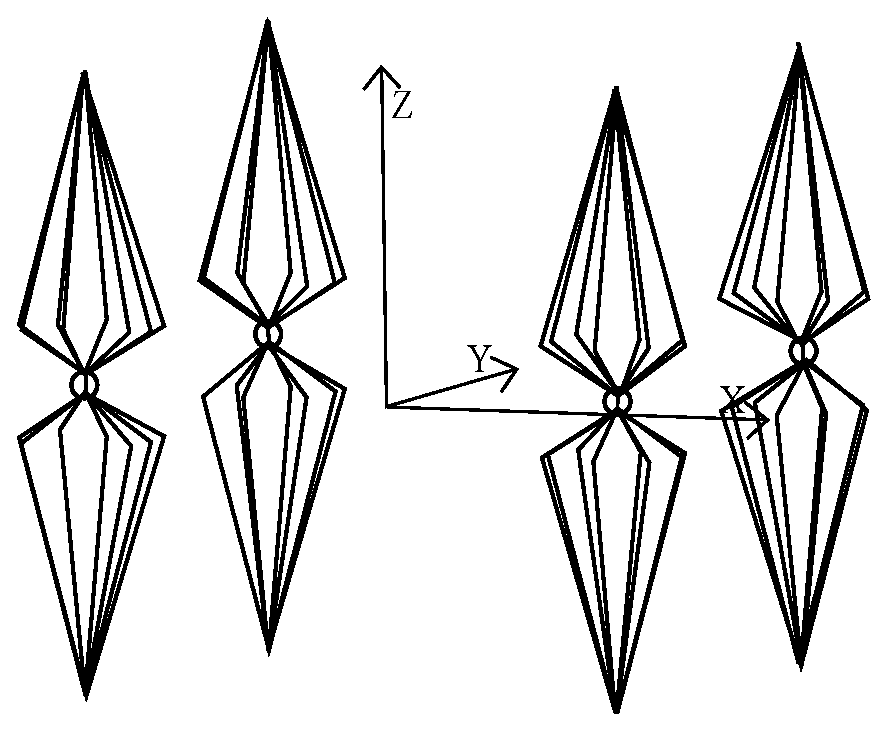
\includegraphics[width=0.6\linewidth]{2x2bvd.eps} \\ б)}
    \end{minipage}
    \begin{minipage}[h]{0.49\linewidth}
        \center{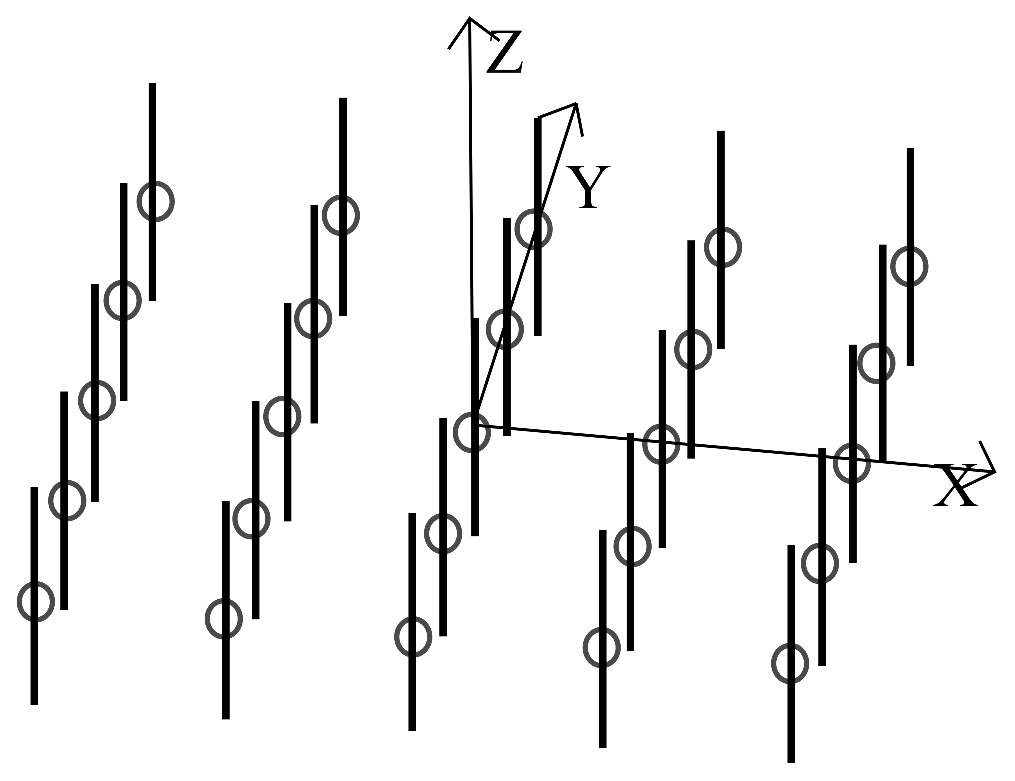
\includegraphics[width=0.6\linewidth]{5x5SVD.eps} \\ в)}
    \end{minipage}
    \hfill
    \begin{minipage}[h]{0.49\linewidth}
        \center{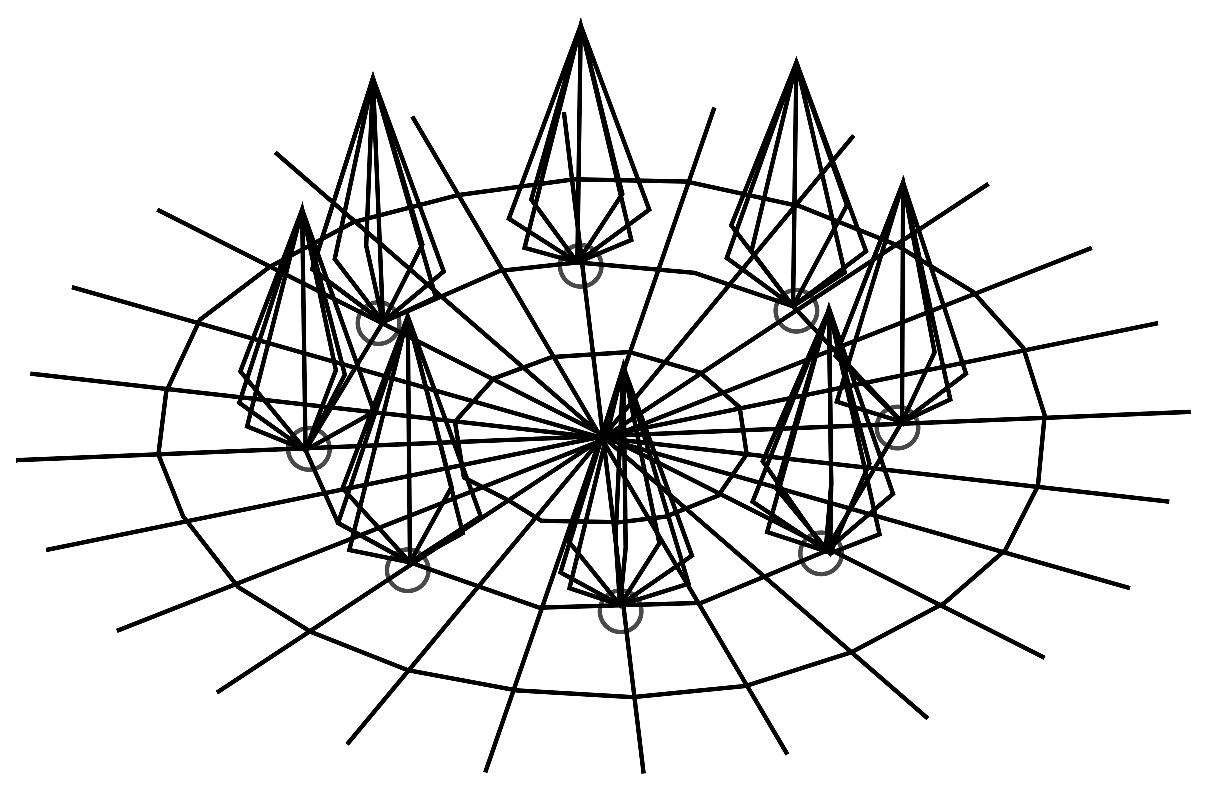
\includegraphics[width=0.9\linewidth]{r8.eps} \\ г)}
    \end{minipage}
    \caption{ФАР различных конфигураций}
    \label{ris:bve_bvd}
\end{figure}


\section{Постановка задачи}\label{sec:statement}

Нашей задачей является максимизация излучения антенной решетки в заданном направлении при ограничениях на мощность, подводимую к каждому
излучателю. В терминах комплексных токов, подводимых к излучателям, эта задача сформулирована в работах~\cite{yurkov:farkv,yurkov:knd}.
Пусть $l$ - индекс компоненты вектора направления: $l=1$ для азимутального и $l=2$ для полярного угла. Расстояние до приемника принимается во много раз превышающим размеры ФАР, поэтому индекс $l$ итерирует только эти два значения.
Суммарное электромагнитное поле $f^{(l)}_{\Sigma}$, выраженное в комплексных единицах, вводится как
%
\begin{equation}
    f^{(l)}_{\Sigma} = \sum_{i=1}^{N}I_i \tilde{f}_i^{(l)} \, ,
    \label{eq:sumfield}
\end{equation}
%
где $N$ - число точек питания антенной системы, $I_i$ - комплексный ток в $i$-й точке питания; $\tilde{f}_i^{(l)}$ - парциальное поле, то есть поле, которое излучается при подаче единичного тока на $i$-ю точку питания излучающей системы, в то время, как ток в других точках питания равен нулю. В качестве количественной меры оценки электромагнитного поля используется напряженность электрического поля. Отметим, что из определения парциального поля следует, что $\tilde{f}_i^{(l)}$ имеет размерность поля, нормированного к току. Справедливость выражения~(\ref{eq:sumfield}) следует из линейности уравнений Максвелла (более подробно см.~\cite{yurkov:farkv}). Таким образом, суммарное поле $f^{(l)}_{\Sigma}$ является суперпозицией парциальных полей от каждой точки питания излучающей системы.

Значения $f_i^{(l)}$ и $f^{(l)}_{\Sigma}$ - функции направления и частоты, которые могут быть вычислены с помощью некоторой программы моделирования антенн (здесь мы используем NEC-2~\cite{bruke:nec2}).

За $\overline{f}$ обозначим комплексное сопряжение к $f$. Как было упомянуто выше, цель - максимизация направленности излучения. В качестве количественной меры оценки направленности излучения понимается плотность мощности поля в заданном направлении, обозначаемая через $F$. Через компоненты электромагнитного поля $F$ выражается по формуле~(\ref{eq:FPrimary})
%
    \begin{equation}
        F = \sum_{l=1}^{2}\overline{f}_{\Sigma}^{(l)}f_{\Sigma}^{(l)}
        \label{eq:FPrimary}
    \end{equation}
%
и является целевой функцией задачи. При максимизации $F$ необходимо учитывать ограничения на активную мощность, которую способны выдавать усилители, питающие антенную систему. В силу закона Ома такие ограничения могут быть выражены в терминах только токов или только напряжений. Чтобы найти мощность $i$-го источника, мы вводим соответствующие комплексные напряжения~$U_i$ следующим образом:
%
    \begin{equation}
        I_i = \sum_{j=1}^{N}y_{ij}U_j \, ,
        \label{eq:om}
    \end{equation}
%
где $y_{ij}$ - элементы матрицы проводимостей $\textbf{Y} = (y_{ij})$, имеющей размерность $N \times N$.

В некоторых случаях более удобно использовать матричную нотацию. В рамках данной нотации мы вводим вектор-столбец токов $\textbf{i}$ и вектор-столбец напряжений $\textbf{u}$, состоящие из $N$ элементов. Целевая функция в таком случае формулируется следующим образом:
%
    \begin{equation}
        F = \textbf{u}^{+}\textbf{Au} \, ,
        \label{eq:F}
    \end{equation}
%
где верхний индекс $+$ означает эрмитово сопряжение, $A = (a_{ij})$,
%
     \begin{equation}
        a_{ij} = \sum_{l=1}^2\overline{f}_{i}^{(l)}f_{j}^{(l)}
        \label{eq:A} \, .
    \end{equation}
%
Соответственно, соотношение между токами и напряжениями записывается следующим образом:
%
    \begin{equation}
    \textbf{i}=\textbf{Y}\textbf{u} .
    \end{equation}
%

Существуют различные формы ограничений, которые соответствуют различным антенным системам. Например, можно ограничить суммарную мощность $P$ по всем точкам питания. В этом случае задача оптимизации формулируется так:
%
     \begin{equation}
        \begin{cases}
           \textbf{u}^{+}\textbf{Au} \rightarrow \max,\\
           \textbf{u}^{+}\textbf{Bu} = 1,
         \end{cases}
         \label{eq:task1}
    \end{equation}
%
где
%
    \begin{equation}
        \textbf{B} = \frac{1}{4P}(\textbf{Y} + \textbf{Y}^{+}).
        \label{eq:B}
    \end{equation}
%
Такая задача может быть решена аналитически~\cite{yurkov:farkv}.

Задача усложняется, когда ограничение на мощность накладывается по каждой точки питания. В этом случае задача формулируется в виде:
%
    \begin{equation}
        \begin{cases}
           \textbf{u}^{+}\textbf{Au} \rightarrow \max,\\
           0 \leq \textbf{u}^{+}\textbf{B}^{(1)}\textbf{u} \leq 1, \\
           ...\\
           0 \leq \textbf{u}^{+}\textbf{B}^{(n)}\textbf{u} \leq 1,\\
           \textbf{u} \in \mathbb{C}^N\\
         \end{cases}
         \label{eq:task2}
    \end{equation}
%
где $\mathbb{C}$ - поле комплексных чисел, $n$ - число точек питания, на которые накладываются ограничения (в общем случае $n$ может быть не равно $N$),
%
    \begin{equation}
        \textbf{B}^{(k)} = \frac{1}{4P_{max}^{(k)}}(\textbf{Y}^{+}\mathcal{P}^{(k)} + \mathcal{P}^{(k)}\textbf{Y}) \, ,
    \end{equation}
%
$P_{max}^{(k)}$ - максимально допустимая мощность в $k$-й точке питания, $\mathcal{P}^{(k)}$ - матрицы-проекторы имеющие единственный ненулевой элемент $\mathcal{P}^{(k)}_{kk}=1$. Матрицы-проекторы имеют размерность $N \times N$.

Доказано \cite{yurkov:farkv}, что:
%
\begin{enumerate}
  \item Все матрицы $\textbf{B}^{(k)}$ имеют не больше чем два ненулевых собственных значения. Одно из собственных значений положительно,
  остальные отрицательные или нулевые.
  \item Матрицы $\textbf{A}$ и $\textbf{B}^{(k)}$ эрмитово-самосопряженные, то есть
  $a_{ij} = \overline{a}_{ji}$ для всех $i = \overline{1,N}, j = \overline{1,N}$.
  \item Матрица $\textbf{A}$ положительно полуопределена.
  \item Кроме того, из физических соображений вытекает, что матрица $\textbf{B}_{\sum}:= \sum_{k=1}^{n} \textbf{B}^{(k)}$
  положительно определена, так как суммарная активная мощность, поглощаемая пассивной цепью, не может быть отрицательной либо нулем,
  поскольку, часть энергии обязательно излучится~\cite{yurkov:farkv}.
\end{enumerate}

\section{Методы решения}

В данной работе мы рассматриваем подход к решению задачи максимизации направленности излучения ФАР в заданном направлении при ограничениях, накладываемых на мощность, подаваемую на каждый из излучателей. Такая задача может быть решена только численными методами~\cite{yurkov:farkv}. Для использования градиентного метода задача сводится к задаче безусловной оптимизации методом штрафных функций. Выбор градиентного алгоритма связан с тем, что отыскание даже локального оптимума в задаче невыпуклого квадратичного программирования может представлять собой NP-трудную задачу, и одним из методов, уместных в таких случаях, является градиентный алгоритм~\cite{murty:np}. Согласно~\cite{nesterov:nonconvex}, использование метода сопряженных градиентов для решения данной задачи не будет приводить к существенным улучшениям по сравнению с простым градиентным подъемом. Данное утверждение нашло согласие с результатами предварительных вычислительных экспериментов, проведенных нами для некоторых из рассматриваемых задач.

Для оценки качества результатов градиентного алгоритма производится их сравнение с решениями, полученными с помощью решателя
BARON в пакете GAMS. BARON использует алгоритмы метода ветвей и границ, усиленные различными методами распространения ограничений и двойственности для уменьшения диапазонов переменных в ходе работы алгоритма~\cite{ryoo:nlp}. Его использование также представляет альтернативный подход к решению данной задачи, но, поскольку BARON является коммерческим решателем, произведение расчетов требует приобретения лицензии, что не всегда приемлемо.

Еще одним эффективным подоходом к решению невыпуклых задач квадратичного программирования являются генетические алгоритмы, и, в частности, методы дифференциальной эволюции (ДЭ)~\cite{storn:de,noguchi:de}. Использование методов ДЭ требует больше времени, чем использование градиентного подъема, однако, в отличие от градиентных методов, не требует вычисления производных и не подвержен преждевременному завершению в точках стационарности. Таким образом, методы ДЭ также могут быть применены при исследовании структуры локальных оптимумов задачи невыпуклого квадратичного программирования.

Вообще говоря, при использовании метода градиентного подъема не гарантируется получение глобального оптимума. Приблизиться к глобальному
оптимуму позволяет многократный запуск алгоритма из случайным образом сгенерированных точек. Кроме того, многократный запуск позволяет
оценить количество локальных оптимумов, что является некоторым критерием сложности индивидуальной задачи~\cite{eremeev:confidence}. Анализ структуры локальных оптимумов позволяет также выявить наличие нетривиальных симметрий.


\section{Формулировка задачи в действительных числах} \label{subsec:statement}

Для разработки алгоритма решения задачи удобно переформулировать ее в вещественных числах. Обозначим соответствующие матрицы: $\textbf{G} \in \mathbb{R}^{(2N)^2}$ для целевой функции и $\textbf{H}^{(k)} \in \mathbb{R}^{(2N)^2}; k = \overline{1,n}$ для ограничений. Пусть $\textbf{y} \in \mathbb{C}^N$, $\textbf{A} \in \mathbb{C}^{N^2}$, и пусть $\textbf {x} \in \mathbb{R}^{2N}$ - вектор, где первые $N$
компонент являются вещественными частями соответствующих компонент вектора~$\textbf{y}$, в то время, как остальные компоненты соответствуют мнимым, то есть:
%
    $$
    \textbf{y}_i \in \mathbb{C} \longleftrightarrow (\textbf{x}_i,
    \textbf{x}_{N+i}), \ \textbf{x}_i = Re(\textbf{y}_i), \
    \textbf{x}_{N+i} = Im(\textbf{y}_i) \, i = \overline{1,N}.
    $$
%
Через $\textbf{G} \in \mathbb{R}^{(2N)^2}$ обозначим матрицу следующего вида:
%
    \begin{equation}
        \left( \begin{array}{c | c}
            Re(\textbf{A})& -Im(\textbf{A})\\
            \hline
            Im(\textbf{A})& Re(\textbf{A})\end{array}
        \right) .
    \end{equation}
%
Легко проверить, что
    \begin{equation}
        \left(\begin{array}{c} Re(\textbf{Ay}) \\ Im(\textbf{Ay})\end{array} \right) =
        \textbf{G}\left(\begin{array}{c} Re(\textbf{y}) \\ Im(\textbf{y})\end{array}\right) .
    \end{equation}
%

Из того, что матрица $\textbf{A}$ эрмитово-самосопряженная, следует, что матрица $\textbf{G}$ симметричная. Действительно, так как матрица $\textbf{A}$ эрмитово-самосопряжена, следует симметричность $Re(\textbf{A})$ и кососимметричность $Im(\textbf{A})$. Это значит, что
%
    $$
        \textbf{G}^T = \left( \begin{array}{c | c}
            Re(\textbf{A}) & (Im(\textbf{A}))^T \\
            \hline
            (-Im \textbf{A})^T & Re(\textbf{A}) \end{array}
        \right) = \left( \begin{array}{c | c}
            Re(\textbf{A}) & -Im(\textbf{A}) \\
            \hline
            Im(\textbf{A}) & Re(\textbf{A}) \end{array}
        \right)= \textbf{G} \, .
    $$
%
Таким образом, $\textbf{G}$ является симметрической матрицей. То же самое применимо к матрицам ограничений $\textbf{H}^{(k)} \in \mathbb{R}^{(2N)^2}; k=\overline{1,n}$. В вещественных числах задача~(\ref{eq:task2}) эквивалентна следующей:
    \begin{equation}
        \begin{cases}
           \textbf{x}^{T}\textbf{Gx} \rightarrow \max,\\
           0 \leq \textbf{x}^{T}\textbf{H}^{(1)}\textbf{x} \leq 1,\\
           ...\\
           0 \leq \textbf{x}^{T}\textbf{H}^{(n)}\textbf{x} \leq 1,\\
          \textbf{x} \in \mathbb{R}^{2N}.\\
         \end{cases}
         \label{eq:task3}
    \end{equation}

Задача~(\ref{eq:task3}) имеет целевую функцию, заданную квадратичной формой с положительно полуопределенной матрицей~$\textbf{G}$. Каждое ограничение формулируется квадратичной формой, определенной симметричной матрицей~$\textbf{H}^{(k)}, k=\overline{1,n}$ с двумя парами идентичных собственных значений, два из которых положительны, а другие два отрицательны или равны нулю, все остальные собственные числа равны нулю.

Следует отметить, что задача~(\ref{eq:task2}), сформулированная в комплексных числах, имеет симметрию относительно преобразования $\textbf{u} \to e^{\emph{\textbf{j}}\phi}\textbf{u}$ всех комплексных координат (по произвольному углу~$\phi$). За $\emph{\textbf{j}}$ здесь обозначена мнимая единица. В качестве доказательства рассмотрим некоторую квадратичную форму, определенную матрицей \textbf{M}: $${(\textbf{v}e^{\emph{\textbf{j}}\phi})}^{+}\textbf{M}(\textbf{v}e^{\emph{\textbf{j}}\phi}) =
\sum_{l=1}^{N}\sum_{k=1}^{N}|v_k||v_l|m_{kl}e^{\emph{\textbf{j}}(\phi_l + \phi - \phi_k - \phi)} =$$
$$ = \sum_{l=1}^{N}\sum_{k=1}^{N}|v_k||v_l|m_{kl}e^{\emph{\textbf{j}}(\phi_l - \phi_k)} .$$

Глобально-оптимальное решение задачи невыпуклого математического программирования вида (\ref{eq:task3}) может быть найдено методом
ветвей и границ~\cite{horst:global,tawarmalani:global} или с использованием методов DC программирования~\cite{horst:handbook,strekalovsky:global}. Локально-оптимальное решение задачи может быть найдено средствами градиентной оптимизации или методом Ньютона~\cite{himmelblau:nlp}. В случае большой размерности могут быть применены различные метаэвристики(см.~\cite{eberhart:swarm,storn:de}).

%\section{Другие постановки задачи}
% TODO

\section{Верхняя оценка нормы допустимых решений} \label{subsec:top}

В вычислительных экспериментах бывает полезно ограничить множество допустимых решений задачи шаром или параллелепипедом, так как это позволяет более обоснованно выбрать начальное решение для итерационных методов с мультистартом или сократить перебор в методе ветвей и границ.

Отмеченная симметрия может найти применение для уменьшения размерности области поиска на единицу. Например, фиксируя $Im(y_{N})=0$, что эквивалентно добавлению ограничения $x_{2N}=0$ к задаче~(\ref{eq:task3}).

Кроме того, можно оценить множество допустимых решений в терминах евклидова расстояния до начала координат. Отметим, что если $\textbf{x}$ удовлетворяет всем ограничениям задачи~(\ref{eq:task3}), то
$$
\min\{\textbf{z}^T \textbf{H}_{\sum} \textbf{z} \ : \ \textbf{z}\in
\mathbb{R}^{2N}, \ ||\textbf{z}|| =1\} = \lambda_{\min},
$$
(см. например~\cite{horn:matrix}, глава~1, \S~1.0.2), мы получаем
$$
\textbf{x}^T \textbf{H}_{\sum} \textbf{x} \ge ||\textbf{x}||^2
\lambda_{\min}\ \
$$
и
\begin{equation} \label{eqn:bound}
||\textbf{x}||\le \sqrt{\frac{N}{\lambda_{\min}}}.
\end{equation}

\section{Масштабирование произвольного решения в допустимую область} \label{sec:scaling}

Для данной задачи существует преобразование, позволяющее привести к допустимой области решение $\textbf{x}$, которое нарушает только ограничивающие неравенства задачи~(\ref{eq:task3}) вида $\textbf{x}^{T}\textbf{H}^{(k)}\textbf{x} \leq 1$:

\begin{equation}
    \textbf{x}': =\alpha(\textbf{x})^{-1/2} \textbf{x} ,
    \label{eq:scale}
\end{equation}
где $\alpha(\textbf{x}):=\max_{k=\overline{1,n}} \textbf{x}^T \textbf{H}^{(k)}\textbf{x}$. Поскольку как целевая функция, так и ограничения представлены квадратичными формами, применение такой операции приведет к пропорциональному уменьшению в~$\alpha(\textbf{x})$ раз значений каждой из квадратичных форм. Другими словами, если в некоторой точке $\textbf{x}$ значения каждой из квадратичных форм, задающих ограничения, больше 0, причем значения некоторых из них больше 1, то по формуле (\ref{eq:scale}) можно определить множитель, умножение которого на вектор $\textbf{x}$ ведет к тому, что наибольшее из значений квадратичных форм, задающих ограничения, будет равно 1. Данная процедура применяется для выбора начального решения, а также для масштабирования итогового решения.

Результаты данного раздела были представлены в~\cite{tyu:daor,tyu:opta,tyu:fmh}.